\documentclass[t]{beamer}
\usetheme{CambridgeUS}

\usepackage{minted}
\usepackage{colortbl}

\title{Practical Parallelism}
\author{Jaimie Murdock}
\institute[IU COGS]{
    IU Cognitive Science Program\\
    810 Eigenmann Hall\\
    \texttt{jammurdo@indiana.edu}
    }
\date{November 17, 2011}

\begin{document}
% Title Page
\frame{\titlepage}
\frame{\tableofcontents}

\section{Introduction}
\subsection{Motivation}
\begin{frame}
\frametitle{Motivation}
Multiprocessing has moved from HPC-only to SMP
% TODO: Find chart of intel desktop shipments
\pause \bigskip

Cores are cheap:
\tiny{
\begin{itemize}
  \item \textbf{2} -- Intel Celeron E3400 -- \$47
  \item \textbf{4} -- AMD Athlon II X4 631 -- \$90
  \item \textbf{6} -- AMD Phenom II X6 1035T -- \$135
  \item \textbf{8} -- AMD FX-8120 -- \$210
\end{itemize}}

\pause \bigskip

The rise of the cloud --- clusters for everyone
% TODO: Insert Google App Engine, Amazon Web Services, Microsoft Azure
\end{frame}

\begin{frame}
\frametitle{How fast?}
\begin{center}
  \textbf{Amdahl's Law} \\
  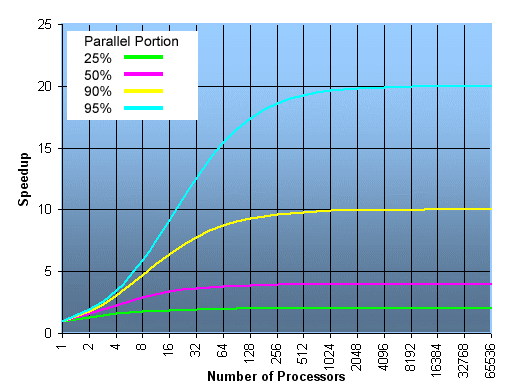
\includegraphics[width=0.7\textwidth]{img/amdahl2.png} 
\end{center}
\end{frame}

\subsection{Basics}[fragile]
\begin{frame}
\frametitle{Painfully Parallel Problems}
(or: how to use C211 in an interview)\\
\pause

Given a function that is both commutative and associative (e.g., $+$ or $*$)\\
\pause
\begin{itemize}
  \item \textbf{Commutative:} $x + y = y + x$ \\
  \item \textbf{Associative:} $(x + y) + z = x + (y + z)$
\end{itemize}

% TODO: fix table
%$MapReduce(+, 5 6 4 1 4 1 2 5 6 2 7 6 3 4 6 1)$
\begin{tabular}{rcccc}
Partition: & 5 6 4 1 & 4 1 2 5 & 6 2 7 6 & 3 4 6 1 \\ 
Map:       & 16 & 12 & 21 & 14 \\
Reduce:    & 63 & & & \\
\end{tabular}
\end{frame}

% TODO: Insert OpenMP C reduction

\begin{frame}
\frametitle{Painfully Parallel Problems}
\begin{center}
  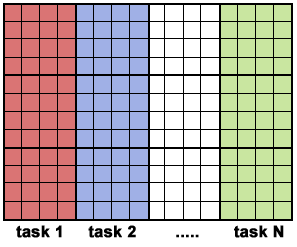
\includegraphics[width=0.7\textwidth]{img/array.png} 
\end{center}
\end{frame}


\begin{frame}
\frametitle{Painfully Parallel Problems}
\begin{center}
  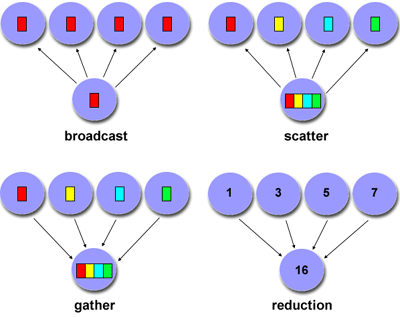
\includegraphics[width=0.7\textwidth]{img/problems.png} 
\end{center}
\end{frame}

\begin{frame}
\frametitle{Architecture}
\textbf{Flynn's Taxonomy}
\begin{itemize}
\item SISD -- Single Instruction, Single Data
\end{itemize}

\begin{center}
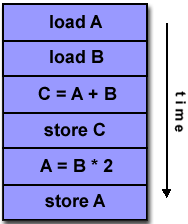
\includegraphics[width=0.3\textwidth]{img/sisd.png} 
\end{center}
\end{frame}

\begin{frame}
\frametitle{Architecture}
\textbf{Flynn's Taxonomy}
\begin{itemize}
\item SISD -- Single Instruction, Single Data

\item SIMD -- Single Instruction, Multiple Data
%\footnotesize{MMX, SSE, AltiVec, 3dNow!, GPU}
\end{itemize}

\begin{center}
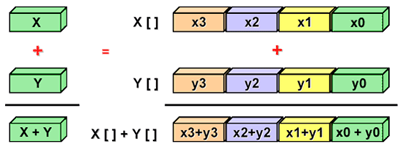
\includegraphics[width=0.6\textwidth]{img/simd.png} 
\end{center}
\end{frame}
\begin{frame}
\frametitle{Architecture}
\textbf{Flynn's Taxonomy}
\begin{itemize}
\item SISD -- Single Instruction, Single Data

\item SIMD -- Single Instruction, Multiple Data
%\footnotesize{MMX, SSE, AltiVec, 3dNow!, GPU}

\item MISD -- Multiple Instruction, Single Data 
%\footnotesize{multiple filters}
\end{itemize}

\begin{center}
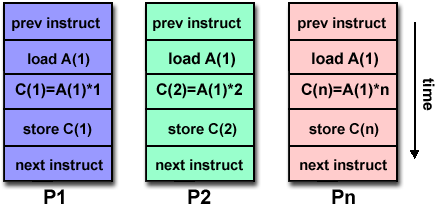
\includegraphics[width=0.6\textwidth]{img/misd.png} 
\end{center}
\end{frame}
\begin{frame}
\frametitle{Architecture}
\textbf{Flynn's Taxonomy}
\begin{itemize}
\item SISD -- Single Instruction, Single Data

\item SIMD -- Single Instruction, Multiple Data
%\footnotesize{MMX, SSE, AltiVec, 3dNow!, GPU}

\item MISD -- Multiple Instruction, Single Data 
%\footnotesize{multiple filters}

\item MIMD -- Multiple Instruction, Multiple Data
%\footnotesize{true multiprocessing}
\end{itemize}

\begin{center}
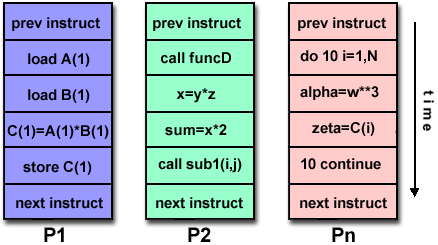
\includegraphics[width=0.6\textwidth]{img/mimd.png} 
\end{center}
\end{frame}
\subsection{Synchronization}
\begin{frame}
\frametitle{Synchronization}
\begin{tabular}{cc}
\textbf{Process 1} & \textbf{Process 2} \\
$a = read(A)$    & $a = read(A)$ \\
$a = a + 1$      & $b = read(B)$ \\
$A = write(a)$   & $A = write(a +b)$
\end{tabular}

\pause
\bigskip

Solutions:
\begin{itemize}
  \item Barriers
  \item Locking
  \item Semaphores
\end{itemize}

\end{frame}


% TODO: Insert C example

\begin{frame}[fragile]
\frametitle{Locks}
\textbf{C\#}
\begin{minted}[fontsize=\footnotesize]{csharp}
class Account {     // this is a monitor of an account
  long val = 0;
 
  public void Deposit(const long x) {
    lock (this) {   // only 1 thread at a time may execute this statement
      val += x;
    }
  }
 
  public void Withdraw(const long x) {
    lock (this) {
      val -= x;
    }
  }
}
\end{minted}
\end{frame}

\begin{frame}[fragile]
\frametitle{Locks}
\textbf{Java}
\begin{minted}[fontsize=\footnotesize]{java}
class Account {     // this is a monitor of an account
  int val = 0;
 
  public synchronized void Deposit(int x) {
    val += x;
  }
 
  public synchronized void Withdraw(int x) {
    val -= x;
  }
}
\end{minted}
\end{frame}

\begin{frame}[fragile]
\frametitle{Locks}
\textbf{Python}
\begin{minted}[fontsize=\footnotesize]{python}
from threading import Lock
class Account:
    def __init__(self, value):
        self.value = value
        self.lock = Lock()

    def deposit(x):
        with self.lock:
            self.value += x

    def withdraw(x):
        with self.lock:
            self.value -= x
\end{minted}
\end{frame}

\begin{frame}
\frametitle{Memory Models}
\begin{columns}
\begin{column}{.4\textwidth}
\textbf{Shared Memory}
\begin{itemize}
  \item Same address space
  \item Multithreading
\end{itemize}
\end{column}

\begin{column}{.6\textwidth}
\begin{center}
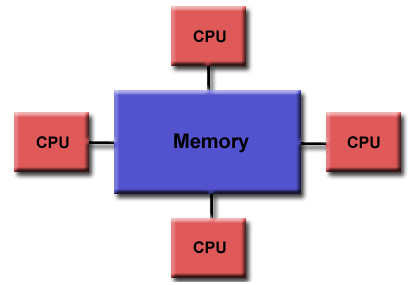
\includegraphics[width=0.8\textwidth]{img/shared_mem.png} 
\end{center}
\end{column}
\end{columns}
\end{frame}


\begin{frame}
\frametitle{Memory Models}
\begin{columns}
\begin{column}{.4\textwidth}
\textbf{Shared Memory}
\begin{itemize}
  \item Same address space
  \item Multithreading
\end{itemize}

\textbf{Distributed Memory}
\begin{itemize}
  \item Different address space
  \item Cluster computing/HPC
\end{itemize}
\end{column}

\begin{column}{.6\textwidth}
\begin{center}
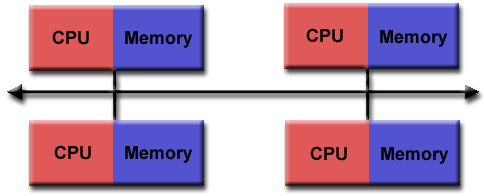
\includegraphics[width=1.0\textwidth]{img/distributed_mem.png} 
\end{center}
\end{column}
\end{columns}
\end{frame}

\begin{frame}
\frametitle{Memory Models}
\begin{columns}
\begin{column}{.4\textwidth}
\textbf{Shared Memory}
\begin{itemize}
  \item Same address space
  \item Multithreading
\end{itemize}

\textbf{Distributed Memory}
\begin{itemize}
  \item Different address space
  \item Cluster computing/HPC
\end{itemize}

\textbf{Hybrid Shared-Distributed Memory}
\begin{itemize}
  \item Multiprocessing
  \item GPU Programming
\end{itemize}
\end{column}

\begin{column}{.6\textwidth}
\begin{center}
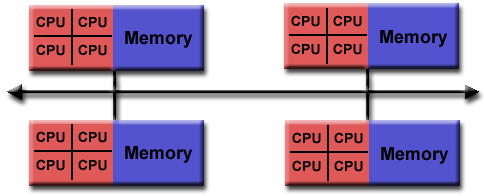
\includegraphics[width=1.0\textwidth]{img/hybrid_mem.png} 
\end{center}
\end{column}
\end{columns}
\end{frame}


% TODO: Insert OpenMP keywords

\begin{frame}
\frametitle{Threads vs. Processes}
\textbf{Threads}
\begin{itemize}
  \item Shared memory
  \item Single process (core), multiple execution paths
  \item Subroutines, GUIs
  \item Low OS overhead
  \item Requires synchronization
  \item POSIX threads, Python \texttt{threading}, Java \texttt{java.lang.Thread}
\end{itemize}

\textbf{Process}
\begin{itemize}
  \item Distributed memory
  \item Message passing
  \item High OS overhead
  \item Only way to utilize multicore or clusters
\end{itemize}

\end{frame}

\begin{frame}
\frametitle{Pipes and Queues}
\textbf{Queue}
\begin{itemize}
  \item Bianry communication of messages
  \item I/O across processes
\end{itemize}

\pause

\textbf{Pipe}
\begin{itemize}
  \item One-way communication of messages. 
  \item Useful for handling I/O to multiple processes
\end{itemize}
\end{frame}



\section{Libraries}

\subsection{MapReduce}
\begin{frame}
\frametitle{MapReduce}
2004 Google framework\\
\texttt{\url{http://labs.google.com/papers/mapreduce.html}}\\
\textbf{APIs}: C++, C\#, Erlang, Java, OCaml, Perl, Python, PHP, Ruby, F\#, R

\pause \bigskip

Six-stage pipeline:
\begin{itemize}
  \item input reader
  \item map function
  \item partition function
  \item comparison function
  \item reduce function
  \item output writer
\end{itemize}
\end{frame}

\begin{frame}[fragile]
\frametitle{MapReduce}
\begin{minted}[fontsize=\footnotesize]{java}
void map(String name, String document):
  // name: document name
  // document: document contents
  for word in document:
    EmitIntermediate(word, "1");
 
void reduce(String word, Iterator partialCounts):
  // word: a word
  // partialCounts: a list of aggregated partial counts
  int sum = 0;
  for pc in partialCounts:
    sum += ParseInt(pc);
  Emit(word, AsString(sum));
\end{minted}
\end{frame}

% TODO: Insert Process Pools and Workers

\subsection{Hadoop}
\begin{frame}
\frametitle{Hadoop}
% TODO: Insert logo
\textbf{The Big Concepts}
\medskip
\begin{itemize}
  \item \textbf{JVM} -- Implemented in Java, commonly used with Clojure and Scala
  \pause
  \item \textbf{HDFS} -- distributed file system, operates in 64MB chunks.
  \pause
  \item \textbf{Sharding} -- Partitioning. Bring the application to the data to reduce bandwidth
  \pause
  \item \textbf{JobTracker} server takes MapReduce job requests to available \textbf{TaskTracker} nodes. (FIFO process pool!)
\end{itemize}
\end{frame}

% TODO: Fix the column issue so this is on the right side of the previous slide...
\begin{frame}
\frametitle{Hadoop}
\begin{center}
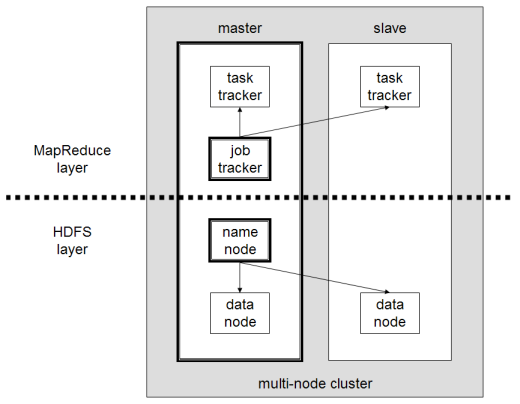
\includegraphics[width=0.5\textwidth]{img/Hadoop_1.png} 
\end{center}
\end{frame}

% TODO: Bandwidth

% TODO: GPU Programming
\begin{frame}
\frametitle{GPU Programming}
\begin{center}
  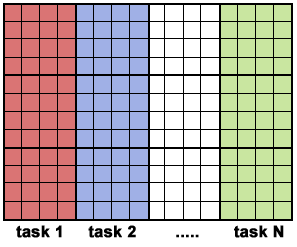
\includegraphics[width=0.7\textwidth]{img/array.png} 
\end{center}
\end{frame}

\begin{frame}
\frametitle{GPU Memory Model}
\begin{center}
  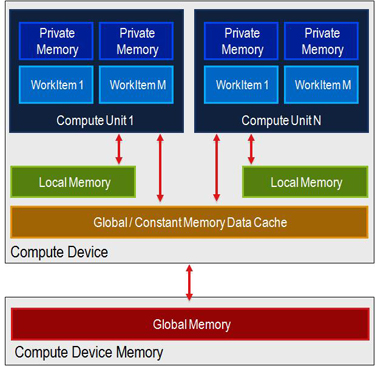
\includegraphics[width=0.5\textwidth]{img/OpenCLMemory.png} 
\end{center}
\end{frame}

\section{Examples}
\subsection{OpenMP}
\begin{frame}[fragile]
\frametitle{OpenMP: Upper Triangular Matrix}
\begin{minted}[fontsize=\footnotesize]{c}
// Calculating Distances
float d; float* D;
for (i = 0; i < POPSIZE; i++) {
    D = dists[i];

    #pragma omp parallel for shared(D, i, dists) private(d, j)
    for (j = i+1; j < POPSIZE; j++) {
        d = distance(i, j);
        D[j] = d;
    }
    
    D[i] = 0.0;
    
    #pragma omp parallel for shared(D, i, dists) private(d, j)
    for (j = 0; j < i; j++) {
        d = dists[j][i];
        D[j] = d;
    }
}
\end{minted}
\end{frame}

\subsection{Python}
\begin{frame}[fragile]
\frametitle{Python \texttt{multiprocessing}}
\begin{minted}[fontsize=\footnotesize]{python}
from multiprocessing import Pool
p = Pool()                  # initialize process pool
results = p.map(f, args)    # spawn processes
p.close()                   # close process pool 
\end{minted}
\end{frame}

\section{Resources}
\begin{frame}
\frametitle{Resources}
\textbf{General}
\begin{itemize}
  \item \url{https://computing.llnl.gov/tutorials/parallel_comp/}
\end{itemize}

\textbf{Python}
\begin{itemize}
  \item \url{http://docs.python.org/library/threading.html}
  \item \url{http://docs.python.org/library/multiprocessing.html} \tiny{Python 2.6}
  \item \url{http://docs.python.org/dev/library/concurrent.futures.html} \tiny{Python 3.2}
\end{itemize}

\textbf{Java}
\begin{itemize}
  \item \url{http://download.oracle.com/javase/7/docs/api/java/lang/Thread.html}
  \item \url{http://download.oracle.com/javase/tutorial/essential/concurrency/}
\end{itemize}
\end{frame}
\begin{frame}
\frametitle{Resources}
\textbf{MapReduce}
\begin{itemize}
  \item \url{http://labs.google.com/papers/mapreduce.html}
  \item \url{http://hadoop.apache.org/}
\end{itemize}
\end{frame}

\begin{frame}
\frametitle{GPU Programming}
\begin{itemize}
  \item \url{http://www.khronos.org/opencl/}
  \item \url{http://developer.amd.com/zones/openclzone/}
  \item \url{http://developer.amd.com/sdks/AMDAPPSDK/samples/}
  \item \url{http://developer.nvidia.com/opencl}
  \item \url{http://developer.nvidia.com/category/zone/cuda-zone}
\end{itemize}
\end{frame}

\frame{\tableofcontents}

\frame{\titlepage}

\end{document}
